\section{Design}\label{sec:design}
Naively vectorizing arbitrary arithmetic circuits looks a lot like SLP: We start by serializing the circuit into a sequence of scalar three-address code.
At each step, we look at all available scalar instructions (i.e. instructions whose operands have all already been scheduled), pick the largest set with the same operation, and schedule them together.
The problem with this naive strategy is it makes no guarantees about values being computed and used on the same lane; in other words, it incurs arbitrarily many shuffles to make the computation line up.
Unlike in normal vectorization, where applying arbitrary permutations to the lanes is relatively cheap, in FHE we are only allowed to rotate the entire vector by a fixed number of slots, and this rotation operation is expensive.
Hence, the cost of bookkeeping quickly outweighs whatever benefit we might get from vectorization, making this approach not worth it.

Data movement is actually impossible to avoid: in an arithmetic circuit that computes a single expression, all the intermediate nodes eventually feed into the root, meaning that without data movement every instruction must be on the same lane; in other words, no vectorization can take place.
Here we have two extremes: on one end of the spectrum is SLP, which packs aggressively without considering data movement; the other end avoids data movement entirely, precluding any vectorization within individual expressions.
The key idea of our approach is to balance between these two extremes, by finding highly vectorizable subexpressions and evaluating them together with each one on its own lane.
% don't be specific about trees here
\subsection{Selecting Vectorizable Subexpressions} 
\subsubsection*{Measuring subexpression vectorizability}
We want to measure how well the instruction sequences corresponding to two arbitrary expressions line up.
Given an arithmetic circuit, we can inductively compute the structural similarity between every pair $(t_1, t_2)$ of independent subcircuits (two circuits are independent if they have no overlap) as follows:

\begin{align*}
    sim(t_1, var) &= 0\\
    sim(var, t_2) &= 0\\
    sim(t_1, t_2) &= \max \begin{cases}
        sim(t_1.L, t_2)\\
        sim(t_1.R, t_2)\\
        sim(t_1, t_2.L)\\
        sim(t_1, t_2.R)\\
        sim(t_1.L, t_2.L) + sim(t_1.R, t_2.R) + b\\
        sim(t_1.L, t_2.R) + sim(t_1.R, t_2.L) + b
    \end{cases}
\end{align*}
where $b = 1$ if $t_1.op = t_2.op$ and $b = 0$ otherwise.

For example, in the circuit from Figure~\ref{fig:small-expr-circuit}, we have a similarity score of $2$ between $(ab + c)$ and $(xy + z)$.

% The base case is comparing any tree to a leaf node (a single variable with no operations), in which case the similarity is $0$, as there are no operations that can be packed together.

% In the inductive case of two nontrivial trees, there are six ways they could be lined up: \raghav{TODO: diagram}
% Either root could be lined up with either child of the other tree in four ways. 
% Or, the two roots could line up, giving two ways for their children to line up (left with left and right with right, or left with right and right with left).
% In the first four cases, the similarity score of the two trees is the similarity score of the alignment. 
% In the last two cases, the similarity score of the two trees is the sum of the scores of the aligned children, plus a 1 if the roots have the same operation.
% The final similarity score of the two trees is the maximum possible score out of all six cases. 
% \raghav{This makes no sense even to me, and I was looking at the code when I wrote this.}\milind{Actually, now that I think about it, maybe write this as a set of recurrence relations, a la smith waterman}

\subsubsection*{Choosing maximally vectorizable sets}%\raghav{TODO: add a running example $(ab+c)(xy+z)$}
Not every pair of subexpressions is eligible to be vectorized together, since they have to be independent of each other.
This data can be encoded in an undirected {\em vectorizability graph}, where each subexpression is a vertex, and there is an edge between two vertices if the corresponding subexpressions are independent (and thus vectorizable).
Cliques in this graph correspond exactly to sets of expressions that can all be vectorized together. 
We can further label each edge with the similarity score of the two subexpressions it connects.
Since each similarity score roughly corresponds to the number of instructions that could be packed together, the total weight of a clique represents the total number of operations we save by vectorizing together all the subexpressions contained within. 
There is a subtlety here: we don't just want to take the largest clique in the graph, since this means vectorizing a lot of expressions, which will likely incur several rotates down the line. 
To account for this, we subtract a fixed amount from the weight of each edge; this penalizes large cliques, and ensures that we prioritize finding small cliques of highly vectorizable expressions to avoid doing too many rotations.
% By simply subtracting a fixed amount from the weight of each edge we can penalize large cliques which would incur a much higher rotation overhead, unless the vectorizability of the clique is high enough to be worth it. \milind{Rephrase this: start by explaining why you don't want to just take super big cliques -- it doesn't take into account rotation -- and then explain how you adjust the weights to account for this}
The problem of finding a set of subexpressions to vectorize together reduces to finding a maximal weight clique in this graph, which is easily packaged off to an SMT solver.

This effectively greedily selects a set of expressions to vectorize, which amounts to scheduling the first {\em epoch} of the program, s we want to repeat the process until the entire program has been scheduled.
Repeating the process requires some extra work: whenever a set of subexpressions is selected, each one needs to be ``quotiented out'' of the original program (i.e. collapsed to a new leaf node in the circuit).
Doing so requires that we make two changes to the vectorizability graph:
\begin{enumerate}
    \item All the nodes that were cut out of the circuit (the {\em sub}-subexpressions) need to be eliminated, since they have already been scheduled.
    \item Removing certain subexpressions changes the structure of the larger expressions containing them, and hence changes the similarity of those larger  expressions in the overall circuit. \footnote{This is in contrast to what one might expect when vectorizing at the level of instructions instead of subexpressions. The reason we vectorize at the level of subexpressions is to reduce the total number of epochs, and hence the total number of rotations.} These changes need to be reflected by updating the weights of the vectorizability graph. To handle this more efficiently, we track all the pieces that make up the weight of an edge when computing similarities. These weights can then be updated without having to recompute everything each time. \raghav{How's that?}
\end{enumerate}

Using the circuit from Figure~\ref{fig:small-expr-circuit} as a running example, the maximal weight clique in its vectorizability graph is just the edge connecting $(ab + c)$ and $(xy + z)$ (which from earlier has a weight of 2), so \system selects them to vectorize in the first epoch.
After quotienting them out, the remaining expression is just $(L_1 \times L_2)$ where $L_1$ and $L_2$ correspond to the new leaf nodes the subexpressions get collapsed to.
Since there are no subexpressions here that can be vectorized, \system chooses the whole thing for the second and final epoch.
% A single round of this technique greedily selects the optimal ``breakpoints'' up to which to vectorize before inserting rotations, so we need to iterate until the entire program has been scheduled. \milind{This doesn't make sense to me... I think it'll help to have the overview section already talk about stages, so you can explain this in terms of that.}
% Once a set of breakpoints is selected \raghav{Yeah, this is the first time I'm officially using the word breakpoint so far, I should introduce it earlier. Terminology is {\em hard}.}, they need to be ``quotiented out'' (i.e. each subexpression needs to be replaced by a single leaf node in the expression tree).
% This has two effects on the vectorizability graph: First, all the nodes that appear in the quotient need to be eliminated (including the {\em sub}-subexpressions of the chosen subexpressions), since they are no longer eligible to be vectorized.
% However, removing these subexpressions also affects the similarities of their ancestors, since they now have fewer operations that can be packed together.
% These changes must be reflected by updating the weights of the vectorizability graph.
% To avoid having to recompute all the similarities each time, we store for each edge the list of operations it could pack together; the edge weight can be recovered as the sum of the costs of all of these (in the simplest case, the length). \milind{very confusing...}
% Each time a node is quotiented out, it is removed from each list that contains it; doing so automatically updates all the edge weights to account for its removal.
% \raghav{To deal with point (2) more efficiently, I do a trick where I track all the pieces that make up the weight of an edge, so I can update the weights without having to recompute similarity. I originally tried to write this out, but its kind of confusing. Now that I think about it, though, it seems like more of an implementation detail than anything. Should I still write it out here, or just leave it?}\milind{What you wrote in this comment is sufficient, and it's short enough that it's worth including. It {\em is} sort of an implementation detail, but we can cut it for space if we need to.}
Now, we can repeat the above process of finding a maximal clique and vectorizing it, until eventually all nontrivial cliques have a negative total weight, meaning that there are no more subexpressions that are vectorizable enough to make the rotation costs worth it, so we just emit scalar code for the rest of the program.

\subsection{Instruction Packing}
Given a set of subexpressions to compute in a single epoch of the program, we can align the instructions between subexpressions to actually produce a vector schedule.
It may seem like the solution to this is just sequence alignment, but aligning circuits is actually more complicated than that.
At each step, the number of available children that can be aligned roughly doubles, meaning that the total number of subproblems to solve is exponential in the depth instead of linear. 
This causes the dynamic programming strategy of sequence alignment to quickly blow up.
% Aligning trees is more complicated than a simple sequence alignment, because at each step the number of available children to align roughly doubles, meaning that the total number of subproblems to solve is exponential in the depth instead of linear. 
% \raghav{Is this a good enough explanation for why sequence alignment doesn't work here?}\milind{Don't just say sequence alignment out of the blue. You want to say something like "It may seem like the way to go is sequence alignment but ..."}

Instead of wrangling so many subproblems, we can easily formulate this as an ILP.
We create a variable for each scalar instruction representing its {\em schedule slot}, or the time at which it executes.
We add constraints to require that each instruction be scheduled after all of its dependences have been scheduled, and also to require that two instructions with different operations never be scheduled at the same time. 
Finally, to speed up the search for a solution, we place a bound on the total length of the schedule (in other words, an upper bound on the value of the schedule slot for any scalar instruction).
The bound is initially very loose but we iteratively tighten it until the solver returns UNSAT, meaning no smaller schedule could be found, so the most recent one was the smallest.

% Instead of wrangling so many subproblems, we can easily pass this off to an SMT solver. \milind{Maybe say that you formulate this as an ILP? "pass to an SMT solver" is an implementation decision -- the {\em design} is that you create a bunch of ILP constraints}
% The encoding consists of a variable for each instruction representing when it gets scheduled, as well as constraints that require two instructions scheduled at the same time to have the same operation, and constraints that require the two dependencies of each instruction to be scheduled before it.
% Finally, to speed up the search for a solution, we place a bound on the maximum number of slots in the schedule (i.e. the latest time an instruction can be scheduled).
% This bound is initially very loose, but once a schedule is produced we iteratively tighten it until the solver returns UNSAT, meaning no smaller schedule could be found. 
% To prevent compilation from taking too long, we also set a timeout after which the solver simply returns the best available schedule.
% Of course, this means that the vector schedule is no longer guaranteed to be optimal, but this timeout can be adjusted, allowing for a tradeoff between compilation time and optimality.
% sequence of four figures: (a) dependency graph [2 stages] (b) written out list of constraints (c) colored hypergraph (d) colored dependency graph
\subsection{Lane Placement} 
% \milind{This subsection definitely needs a couple of figures: Fig 1: here's some expressions, here's what a ``dumb'' lane placement looks like, here's what a ``good'' lane placement looks like. Fig 2: Here's some expressions. Here's the set of constraints we need to use to capture lane placement constraints. Here's the hypergraph that we derive from those constraints. Here's what it looks like when colored. See how it looks like the ``good'' lane placement?} \raghav{``Correspond'' is also becoming an overused word}
\raghav{TODO: write the bad vs the good lane placement for this example}
\begin{figure*}
    \begin{subfigure}{0.24\textwidth}
        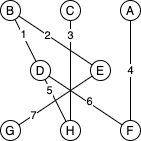
\includegraphics[width=0.9\textwidth]{figures/hypergraph_coloring/small_dependency_graph.drawio.png}
        \caption{A depdendency graph for a simple 3-epoch computation}\label{fig:dependency-graph}
    \end{subfigure}
    \begin{subfigure}{0.24\textwidth}
        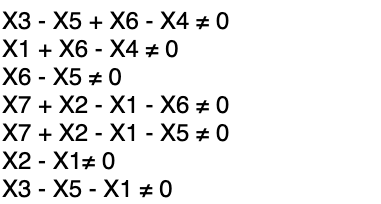
\includegraphics[width=0.9\textwidth]{figures/hypergraph_coloring/hypergraph_relations.drawio.png}
        \caption{The path relations induced by the dependency graph}\label{fig:path-relations}
    \end{subfigure}
    \begin{subfigure}{0.24\textwidth}
        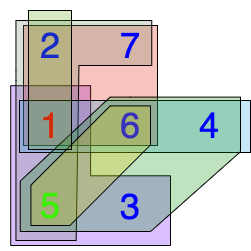
\includegraphics[width=0.9\textwidth]{figures/hypergraph_coloring/colored_dependency_hypergraph.drawio.png}
        \caption{A minimal coloring of the hypergraph corresponding to the path relations}\label{fig:colored-hypergraph}
    \end{subfigure}
    \begin{subfigure}{0.24\textwidth}
        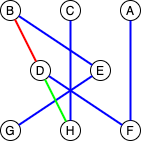
\includegraphics[width=0.9\textwidth]{figures/hypergraph_coloring/colored_dependency_graph.drawio.png}
        \caption{The coloring applied to the original dependency graph. Edges with the same color correspond to the same rotation amount.}\label{fig:colored-dependency-graph}
    \end{subfigure}
    \caption{An example coloring the edges of a dependency graph to produce a good lane assignment}\label{fig:lane-assignment}
\end{figure*}

Once the entire program is scheduled, each epoch produces a set of outputs which may feed into inputs of subsequent epochs.
Since no rotation happens within an epoch, each input must be on the same lane as the output of the epoch it eventually flows into.
This creates a dependence between the output of one epoch with the output of a later epoch, in the sense that if these do not map to the same lane, we need to insert a rotation to line them up.
% Once the entire program is scheduled, each epoch produces a set of outputs which may depend on outputs from previous epochs.
% Each output is produced on a single lane, and whenever a pair of outputs with a dependence between them do not map to the same lane, we need to insert a rotation to get them to line up. \raghav{is this better?}

% Scheduling the program in the way described above amounts to splitting it into a number of {\em epochs}, where each epoch consists of a set of subexpressions to compute. \milind{again ``phase'' vs ``stage''. Also, what's important here isn't that you have the phases -- what's important is that each phase generates output operands in particular lanes, and those operands might need to hook up to one or more input operands in other phases, which means that either the lanes need to be set so everything lines up right, or you need to add rotations.}
For a program that is split into $k$ epochs, we can represent these dependencies in a $k$-partite graph, where each partition corresponds to a epoch and each vertex in a partition corresponds to a subexpression computed in that epoch.
Figure~\ref{fig:dependency-graph} shows an example 3-partite dependency graph for a particular 3-epoch program, where the first epoch had three subexpressions in it, the second had two, and the third had three.
To assign lanes to the subexpressions, we need to assign a number to each vertex in this dependency graph so that no two vertices in the same epoch get the same number.
Unfortunately, a naive approach to this can have very poor results: consider, for example, placing B, D, and G on lane 1, C, E, and F on lane 2, and A and H on the lane 3.
This particular placement requires one rotation each to line up B with E, A with F, and C with H, an additional two rotations to line up D with H and F, and a final rotation to line up E with G.
In the worst case, this incurs 6 rotations.
In the best case, if the vector schedule happens to pack the outputs of B and C together into the same vector, the $B\rightarrow E$ and $C\rightarrow H$ rotations are the same (since they are both a rotation of 1); similarly, if D and E are packed into the same vector, the $D\rightarrow F$ and $E\rightarrow G$ rotations are the same, requiring a total of 4 rotations to line everything up. \raghav{I feel like this is important to say since its the crux of the whole ``use the same number for multiple edges if possible'' thing, but I don't know that I did a good enough job explaining it.}
% This particular placement requires one rotation to line B up with E, an additional two rotations to line D up with H and F, respectively, and a final rotation to line up E with G, incurring a total of four rotations. 
However, if we instead place B, E, and G on lane 1, A, D and F on lane 2, and C and H on lane 3, we can do this with only two rotations: one to line up B and D, and one to line up D and H. 
The goal of the algorithm described here is automatically determining the latter placement.

The heuristic approach is to place vertices on lanes while getting as many edges as possible to have the same rotation along them.
It would be much easier to reason about this by assigning rotation values to edges instead of assigning lanes to vertices, but there is a subtlety we need to keep track of here: not every assignment of rotation values to edges comes from a consistent assignment of lanes to vertices.
This consistency requirement be reworded as follows: for any path that starts and ends on the same epoch in the dependency graph, the {\em directed sum} of the rotation values along it should be zero if the path is a cycle, and nonzero otherwise.
(In a directed sum, we assign a direction to each edge, and negate its value if we follow the edge backwards).
Notice that this automatically enforces that two different paths between a pair of vertices should add up to the same value, since any two such paths also form a cycle by inverting one of them, and the cycle needs to add up to 0.
% Instead, we try to assign lanes in a way that minimizes the number of {\em distinct} rotations required for each vector (for example, if multiple pieces of data on the same vector are produced two lanes away from where they are consumed, we can rotate the vector a single time to get them both to line up).
% In other words, given a $k$-partite graph with an integer associated to each vertex, we can assign to each edge the difference of its two endpoints, representing the rotation. 
% To minimize the distinct numbers we have to assign to the edges, we'd like to be able to go backwards: in other words, we want to assign as few numbers as possible to all the edges such that ``integrating'' them gives a consistent assignment of numbers to the vertices.

% This consistency constraint can be reworded as follows: For every path through the $k$-partite graph that starts and ends on the same partition, the directed sum of the edge weights along that path must be 0 if the path is a cycle, or nonzero otherwise.
% (Notice that this automatically enforces the condition that two different paths between a pair of vertices on the same partition must add up to the same value, since concatenating one path with the reversal of the other produces a cycle, which must sum to 0).
% \raghav{If only I could figure out a neat and tidy way to describe this whole process mathematically\dots}

Iterating over all the paths in the graph, we end up with a bunch of linear {\em path relations} as shown in Figure~\ref{fig:path-relations}, where initially all of the $X_i$s are unassigned.
To assign a particular $X_i$, if it is part of a relation where it is the only unassigned variable, its value is fixed to be one that satisfies the relation; otherwise, it can be assigned freely.
This data forms a hypergraph like the one in Figure~\ref{fig:colored-hypergraph}, where the vertices $1,\dots, 7$ correspond to edges in Figure~\ref{fig:dependency-graph}, and each path relation becomes a hyperedge connecting the associated vertices.
In order to find a consistent assignment of rotation values to edges we need to color this hypergraph in such a way that the last vertex to be colored on any hyperedge must be given a distinct color from the rest of the vertices on the hyperedge (this is equivalent to producing a fresh value for the last $X_i$ to be assigned in a path relation, so it can freely be assigned to satisfy the relation). \raghav{Better explanation?}
To minimize the number of distinct rotations needed, we would like to use as few colors as possible.
This is relatively straightforward to do: At each step we pick the vertex that is part of as few ``free'' hyperedges as possible and assign it the next available color, until all the vertices have been colored.
In the example shown in Figure~\ref{fig:colored-hypergraph}, we first assign to $X_3, X_4$, and $X_7$, (hyperdegree 2), then to $X_2$ and $X_6$ (hyperdegree 3), and then to $X_1$ and $X_5$ (hyperdegree 4).
Since $X_1$ is the last vertex to be assigned in the relation $X_2 - X_1 \neq 0$, it must be given a color other than blue, so it gets red, and since $X_5$ is the last to be assigned in the relation $X_3 - X_5 - X_1 \neq 0$, it cannot be red or blue, so it gets green.

Once the vertices of the hypergraph are colored, we can use it to color the edges of the original dependency graph, like in Figure~\ref{fig:colored-dependency-graph}. 
Now, all that remains is getting actual rotation for each color. 
This can be formulated as a simple integer program, with a variable $c_i$ for each color, a variable  $v_j$ for each node in the dependency graph, and a constraint for each edge $(v, v')$ colored $c$ to assert $v - v' == c$.
The way we colored the hypergraph ensures that this integer program is always solvable, and the solution tells us exactly which vector lane each instruction should go on.

\raghav{I debated including the whole ``how do we calculate paths'' thing as well as the whole ``there's too many paths so we guess at a few and hope it works'' thing but decided against it for now, that may be the wrong decision though}\milind{The CEGIS-y approach to finding paths might be a nice thing to add to the implementation section.}